% (c) Jyotirmoy Bhattacharya, 2013
% Email: jyotirmoy@jyotirmoy.net
%
% This work is licensed under a
% Creative Commons Attribution-ShareAlike 3.0 Unported
% License, 
% http://creativecommons.org/licenses/by-sa/3.0/deed.en_US}.
%
%
\newbox\mybox
{
  \parindent0pt
  \null
  \definecolor{color2}{HTML}{b45412}
  \definecolor{color3}{HTML}{b45412}
  % Need XeTeX for this
  \font\titleface="Arial" at 40pt
  \thispagestyle{empty}
  \vfill
  \hfil
  \begin{tikzpicture}[overlay]
    \coordinate (left) at (-.55\paperwidth,0);
    \coordinate (right) at (0.55\paperwidth,0);
    \coordinate (top) at (0,.55\paperheight);
    \coordinate (bottom) at (0,-0.55\paperheight);
    \coordinate (bandstart) at (0,0.15\paperheight);
    \coordinate (bandend) at (0,0.2\paperheight);
    \fill [black!02] (bottom -|left) rectangle (top-|right);
    \draw (-10mm,80mm) node
    {\titleface \textcolor{color3}{
          macroeconomics}};
    \fill [color2] (bandstart -|left) rectangle (bandend -| right);
    \draw (bandstart -|left) node  [xshift = 110mm,yshift=17pt] {\huge
      \textcolor{white}{\textsf{Jyotirmoy Bhattacharya}}};
    \draw (bandstart -|right) node [xshift =
    -25mm,yshift=-10pt]{\small \textcolor{color2}{\textbf{\myversion}}};
    \draw (bottom -|left) node [above right,xshift=0.1\paperwidth,yshift=15mm] {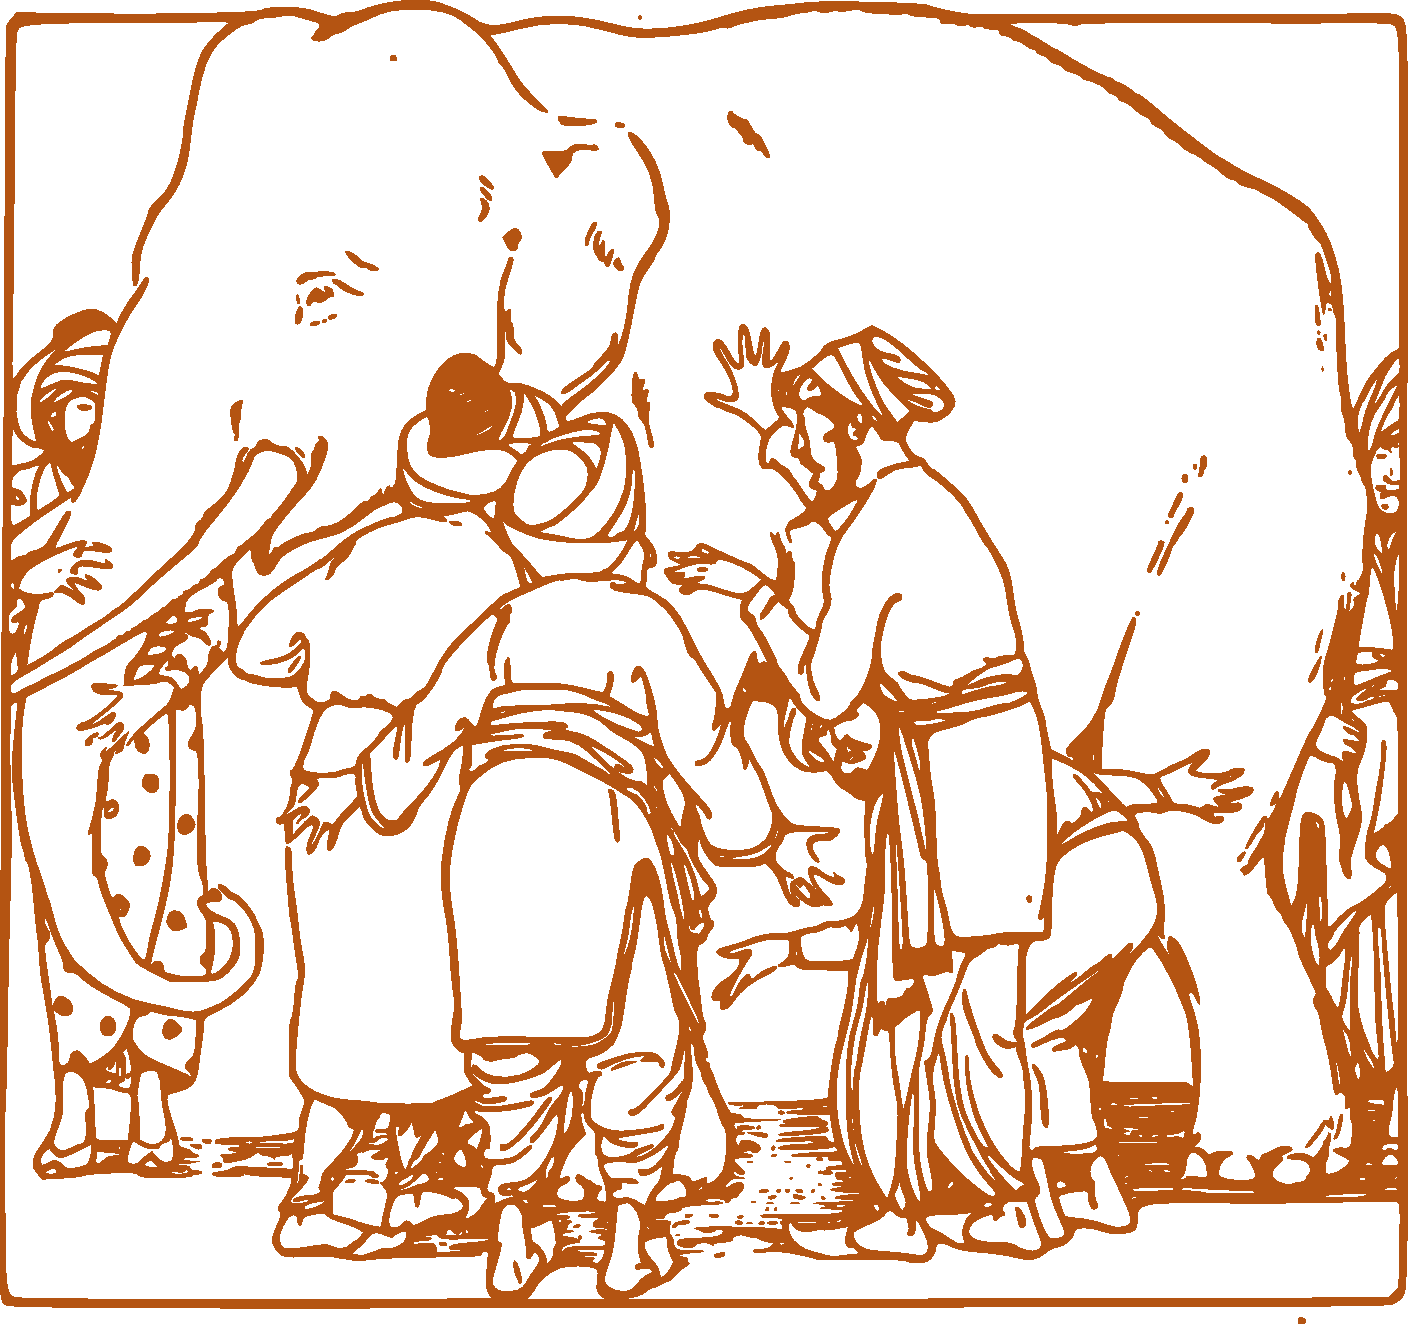
\includegraphics[width=0.8\paperwidth]{coverart/Blind_men_and_elephant.pdf}};
\end{tikzpicture}
\vfill
\vbox{}
}
\clearpage
\thispagestyle{empty}
{
\parindent 0pt
You can find the \LaTeX\ source of this book at
\url{https://github.com/jmoy/jmoy-macroeconomics}
\vfill
\copyright\ Jyotirmoy Bhattacharya, 2013

Email: \texttt{jyotirmoy@jyotirmoy.net}

This work is licensed under a
\href{http://creativecommons.org/licenses/by-sa/3.0/deed.en_US}{Creative
  Commons Attribution-ShareAlike 3.0 Unported License}.
}
\clearpage